\section{Anexo - Diseño de un Acoplador $\pi$}
Como complemento, se solicitó diseñar un acoplador extra para algún tipo de sistema. Se eligió un acoplador de topología $\pi$ para un amplificador de radiofrecuencia.

Se plantea diseñar un acoplador para un receptor que funcione en las frecuencias de AM, con una capacidad de salida de 300pF.

\subsection{Datos}

\begin{itemize}
    \item $P =50W$
    \item $Z_g = 50\Omega$
    \item $Vcc = 24V$
    \item $f_0 = 1120KHz$
    \item $BW = 1170KHz$
    \item $C_o = 300pF$
\end{itemize}

\subsection{Diseño}
Se utilizan las fórmulas de diseño para determinar los valores de los componentes para la siguiente topología.

\begin{figure}[H]
    \centering
    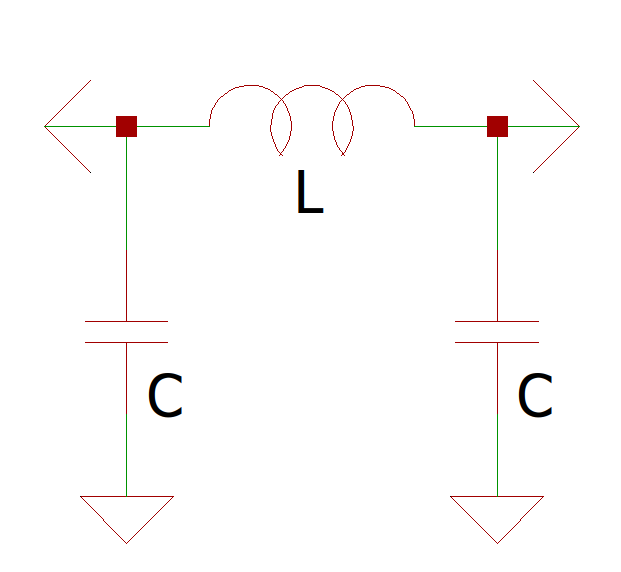
\includegraphics[width=0.5\linewidth]{fig/acopladorpi.png}
    \caption{topología del acoplador pi}
    \label{fig:enter-label}
\end{figure}

$$
Q_c = \frac{f_0}{BW} = 0.96
$$
$$
R'_T = \frac{Vcc^2}{2P_o} = 5.76\Omega
$$
$$
Q_2 = Q_c*2 = 1.92
$$
$$
Q_1 = \sqrt{\frac{R'_T}{R_L}*(1+Q_2^2)} = 0.73
$$
$$
X_{p1} =R_T'/Q_1=7.89\Omega, X_{p2} = Z_L/Q_2 = 26.04\Omega
$$
$$
X_{s1} = \frac{X_{p1}}{1+1/Q_1^2} = 2.74\Omega, X_{s2} = \frac{X_{p2}}{1+1/Q_2^2} = 20.48\Omega
$$
$$
X_s = X_{s1}-X_{s2} = 20.48\Omega-2.74\Omega = 17.74\Omega
$$

Finalmente, la capacidad necesaria para la frecuencia de resonancia del acoplador
$$
C_s = \frac{1}{2\pi1120KHz*17.74\Omega} = 8,01nF
$$
$$
C_p = 300pF+8nF = 8.3nF
$$

El inductor necesario será

$$
L = {\frac{1}{2\pi*f_0}}^2*1/(C_p) = 2.43uHy
$$
